

%\subsection{Fejlesztési lehetőségek a szabályozással kapcsolatban}
%	
%Épületautomatikai rendszerek használatával, például az iContrALL intelligens otthon rendszerével a fellépő zavarásokat (emberek jelenléte, napsütés, szél) mérhetjük. A szabályozás a zavarások hatásmechanizmusának ismeretében jobb zavarelnyomást tud elérni, sőt az integrációval további beavatkozók is használhatók (például árnyékolástechnikai eszközök).
%
%\pagebreak

\chapter{Bevezetés}

\section{Motiváció} A szakdolgozatban elkezdett munkát folytatva a cél az ottani MPC szabályozás finomhangolása, továbbfejlesztése volt. 
A felállított Simulink modellen a szabályozást kvantitatíven vizsgáltam meg, koncentrálva a költségek és a komfort közötti egyensúlyra. 


\section{A modell}
A korábbiakban használt \textit{fűtési rendszer modelljét} nem változtattam meg, viszont a modellből kivezetve mértem a pillanatnyi hőleadást. Így megkaptam a hőmennyiségeket, amik a beavatkozás forintosított költségével arányosak. 


\begin{figure}[H]
	\centering
	% trim={<left> <lower> <right> <upper>}
	%\includegraphics[trim=0 0 0 0, clip,width=\textwidth]{figures/simulink-network-minimalist-layout2}
	\includegraphics[trim=0 0 0 0, clip,width=\textwidth]{figures/simulink-network-minimalist-layout}
	\caption{Fűtési rendszer modellje - fűtőtest és helyiség}
	\label{fig:Simulink-minimalist}
\end{figure}

Adott környezeti hőmérséklet és belső hőmérséklet (alapjel) mellett ez az energiamennyiég azonos volt, mivel a helyiség hőveszteségei csak ennek különbségétől függnek. Az energiamegtakarítást tehát nem itt kell keresni, hanem a primer energia felhasználásánál. Ennek okai a következők:

Az alacsony hőmérsékletű (sugárzó) fűtések, pl. a padlófűtés használata gazdaságosabb lehet a hagyományos radiátoros fűtéseknél a megújulók használatával. Ugyanannyi leadott energia így olcsóbb ilyen rendszerekkel\footnote{Sugárzó fűtésekkel kevesebb primer energia szükséges a jobb hatásfok, kisebb veszteségek miatt.}, emellett pedig jobb hőérzetet biztosítanak.

A modellben a kétféle fűtőtesthez két külön beavatkozó jel tartozik, mely a két szelep kinyitásának mértéke. A beavatkozók dinamikája is eltér, a prediktív irányítás ezt figyelembe véve tud egy egyensúlyt találni.

A csúcsterhelés csökkentése számos előnnyel jár. Szakaszos üzem helyett folyamatos teljesítményigény esetén a megújuló források előnyösebben hasznosíthatók. 

\section{MPC áttekintés}

A modell-prediktív szabályozást alapjaiban a szakdolgozatomban mutattam be. A szabályozó, illetve a zárt szabályozási kör blokkvázlata és a rövidítések magyarázata szerepel az alábbiakban.
\cite{MPCtoolboxGuide} alapján


\begin{figure}[h]
	\centering
	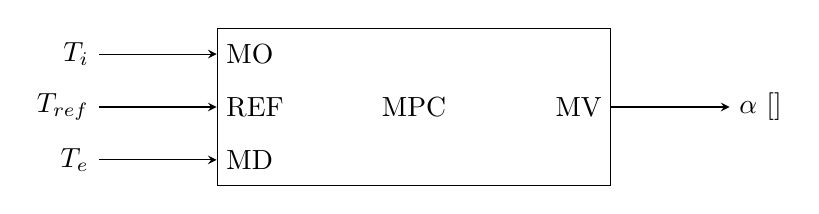
\begin{tikzpicture}[>=stealth]
	% Controller
	% ----------
	\node[draw,rectangle, minimum height=2cm,minimum width=5cm,
		  %label={[xshift=1.0cm, yshift=0.3cm]Label},
		  %label={[xshift=-4.1cm, yshift=-0.7cm]Label},
		  ]
		  (MPC) at (2.3,2.5) {\parbox{2cm}{\centering MPC}};	
	
	% az MPC doboz bemenetei
	\draw [<-] (MPC.165) node[right]{MO} -- +(-15mm,0) node[left]{$T_i$};
	\draw [<-] (MPC.180) node[right]{REF} -- +(-15mm,0) node[left]{$T_{ref}$};
	\draw [->] (MPC.0) node[left]{MV} -- +(15mm,0) node[right]{$\alpha$ [\si{\percent}]};
	\draw [<-] (MPC.195) node[right]{MD} -- +(-15mm,0) node[left]{$T_e$};
	
	\end{tikzpicture}

	\caption{Az MPC be- és kimenetei}
	\label{fig_mpcinout}
\end{figure}

\vspace{6pt}

\begin{table}[H]
	\footnotesize
	\centering
	%\renewcommand{\arraystretch}{2} % to increase cell height
	%\taburulecolor{gray}
	%\begin{tabular}{|p{0.8cm}|p{1cm}|p{1cm}|p{1cm}|p{1cm}|p{1cm}|p{1cm}|p{1cm}|}
	%
	%\begin{tabulary}{\linewidth}{LLc}
	\begin{tabu}{@{}cll@{}}
		\hline
		MPC 	& model predictive control 		& modell-prediktív szabályozás
		\\
		MO / OV	& measured output, output variable 	& mért kimenet (szabályzott jellemző)
		\\
		MD		& measured disturbance			& mért zavarás 
		\\
		MV		& manipulated variable			& beavatkozó jel
		\\
		REF 	& reference signal 				& referenciajel
		\\
		$T_s$ 	& sampling time					& mintavételi idő
		\\ 
		p 		& prediction horizon 			& predikciós horizont 
		\\ 
		c 		& control horizon				& szabályozási horizont
		\\
		J 		& cost function 				& költségfüggvény
		\\
		$w_u$ 	& weight (control signal) 		& beavatkozó jelet büntető együttható
		\\ 
		$w_{\Delta u}$ 	& weight (rate of control signal) 		& beavatkozó jel változását bünteti
		\\ 
		$w_y$ 	& weight (measured output) 		& hibajelet büntető együttható
		\\
		SF 		& scale factor 			& skálázási tényező
		\\    \hline
	\end{tabu}
	\label{tab:mpcoverview}
	\caption{A fejezetben ismertetett rövidítések és angol szakkifejezések}
	%
	%\label{tab:TabularExample}
	%\tabref{TabularExample}~táblázat
\end{table}
\vspace{10pt}


A kiindulási MPC-t már létrehoztam az alábbi lépésekkel:% be kellene tabolni


\begin{enumerate}[noitemsep,topsep=0pt,parsep=2pt,partopsep=4pt,leftmargin=30pt]
	\item a 2 bemenetű, 1 kimenetű szakaszt identifikáltam átviteli függvényével
	\item létrehoztam az MPC-t a megfelelő mintavételi idővel, beállítottam a jelek fizikai korlátait, illetve a skálázást. Az MPC két beavatkozó jele a modell 2 szelepének nyitásához tartozik.
	\item Simulinkben futtatam a szimulációt, Scope használatával mentve az adatokat az analízishez
	
\end{enumerate}


\begin{figure}[H]
	\centering
	% trim={<left> <lower> <right> <upper>}
	%\includegraphics[trim=0 0 0 0, clip,width=\textwidth]{figures/simulink-network-minimalist-layout2}
	\includegraphics[trim=70 0 65 0, clip,width=\textwidth]{figures/onlab/comparepng}
	\caption{Szabályzó szimulációja Simulinkben}
	\label{fig:simulink-mpc}
\end{figure}


\subsection{Az MPC költségfüggvénye}


A szabályzó a predikciós horizonton belül minden lehetséges beavatkozójel-sorozatra kiszámolja annak (várható, modell szerinti) költségét. Azt a beavatkozójel-sorozatot választja, ami a legkisebb költséggel jár. Ez után a szabályozási horizontnak megfelelő számú beavatkozást végez, nem adja ki a teljes sorozatot. 

%A legbutább szabályzó szabályzási és predikciós horizontja is 1. Azaz egy lépéssel lát előre és a legkedvezőbb esethez (J költség minimális) tartozó beavatkozó jelet végrehajtja\footnote{Ezt formalizálni kellene egyenletben is.}. $J=w_u u + w_e e$, ahol a hibát a szabályzóban lévő szakaszmodell alapján számítjuk.
\textit{Agachi \cite{romanMPC_Agachi}} szerint:

\begin{equation} \label{eq_mpc_cost}
J = \sum_{i}^{p} \left(w_u \Delta u^2 + w_e (r_i-y_i)^2  \right)
\end{equation}

%(itt még csak $r_i=r$ állandó referenciajellel tudtam csinálni. )
ahol N a predikciós horizont, $w_u$ a beavatkozó jel változásának súlya, $w_e$ a hibajel súlya. A referenciajel jövőbeli változásait figyelembe lehet venni a predikciós horizonton belül.

A költségfüggvényben a hibajelhez és beavatkozó jelekhez, illetve azok változásaihoz különböző súlyok tartozhatnak.
Nagyobb súlyok nagyobb költséget eredményeznek, így a szabályozó a nagyobb költségű beavatkozójel-sorozatot kisebb valószínűséggel választja.

\chapter{Költség- és komfortoptimum elérése}

\section{OptiControl projekt}
Az ETH Zürich kutatássorozata, az OptiControl \cite{Opticontrol-II} (2007 és 2013 között) a prediktív irányítások használatát vizsgálta és tesztelte irodaépületeken. Az egyetem mellett a Siemens mérnökeit és más partnereket is bevontak. A projektből számos ötletet merítettem, és szimuláltam ezeket a Simulink környezetben.


A projektben MPC szabályozás és RBC (Rule Based Control) performanciáját vetették össze.

Az általuk használt MPC modell meglehetősen részletes: figyelembe veszi a napsütés, illetve az irodában használt elektromos fogyasztók hatását is.

A projekt összefoglalója egy szabályzóval hasonlítja össze a hagyományos megoldásokat, én viszont arra voltam kíváncsi, hogy az általuk használt stratégiák mennyiben befolyásolják az MPC viselkedését.



\section{Peak demand csökkentése}



\subsection{Signal Preview} A prediktív szabályozókban lehetőség van arra, hogy a predikciós horizonton belül a szabályozó figyelembe vegye a referenciajel jövőbeli változását, illetve a mérhető zavarások várható értékét. (Erre previewing vagy look-ahead néven szokás hivatkozni.)


Erre abban az esetben van lehetőség, ha például elő van írva a napi hőmérséklet alapjel, ahogyan ez megtehető egyszerű programozható termosztátoknál is, amelyek egyszerű RBC (Rule Based Control) elven kapcsolnak be vagy ki.


Időjárás-előrejelzést figyelembe véve pedig a külső hőmérséklet értékére adható becslés, ami tovább csökkentheti az energiafelhasználást: Ha a szabályozó csak a pillanatnyi zavarás értékét ismeri, akkor ennek megváltozásakor a referenciajel is hirtelen megváltozhat. Amennyiben a szabályozó a zavarás becsült értékét előre ismeri, optimalizálni tudja az energiafelhasználást. Ha például a külső hőmérséklet hirtelen emelkedik, akkor könnyen túlmelegedhet a helyiség, felesleges energiafogyasztást eredményezve.



\begin{figure}[H]
	\centering
	% trim={<left> <lower> <right> <upper>}
	%\includegraphics[trim=0 0 0 0, clip,width=\textwidth]{figures/simulink-network-minimalist-layout2}
	\includegraphics[trim=10 50 10 0, clip,width=\textwidth]{figures/onlab/preview}
	\caption{Signal previewing hatása (forrás: \cite{BemporadLecture1})}
	\label{fig:preview-bemporad}
\end{figure}

\subsection{Súlyozás módosítása} A költségfüggvényben a beavatkozóknak különböző súlyokat rendelhetünk, ezzel szintén korlátozhatók a beavatkozó jelek. 

A csúcsidőszakban csökkenthető a teljesítményigény, ha a tarifákidőben változnak. Ez elérhető például a súlyok futás közbeni módosításával.

Ezt vizsgálták az \textit{OptiControl projektben} \cite{Opticontrol-II} is, kora reggel és késő este alacsonyabb tarifát feltételezve. (A TABS jelenti a padlófűtést, a Ventilation pedig a légfűtést.)



\begin{figure}[H]
	\centering
	% trim={<left> <lower> <right> <upper>}
	%\includegraphics[trim=0 0 0 0, clip,width=\textwidth]{figures/simulink-network-minimalist-layout2}
	\includegraphics[trim=90 60 90 470, clip,width=\textwidth]{cite/loadshift}
	\caption{Különböző tarifák figyelembe vétele az OptiControl projektben}
	\label{fig:loadshift}
\end{figure}


%\begin{figure}[H]
%	\centering
%	% trim={<left> <lower> <right> <upper>}
%	%\includegraphics[trim=0 0 0 0, clip,width=\textwidth]{figures/simulink-network-minimalist-layout2}
%	\includegraphics[trim=0 0 0 0, clip,width=0.4\textwidth]{figures/onlab/constRefPrev/Cconstref}
%	\caption{C szabályozó}
%	\label{fig:peak2-plottempC}
%\end{figure}
%
%
%\begin{figure}[H]
%	\centering
%	% trim={<left> <lower> <right> <upper>}
%	%\includegraphics[trim=0 0 0 0, clip,width=\textwidth]{figures/simulink-network-minimalist-layout2}
%	\includegraphics[trim=0 0 0 0, clip,width=0.4\textwidth]{figures/onlab/constRefPrev/Cconstref}
%	\caption{C szabályozó}
%	\label{fig:peak2-plottempC}
%\end{figure}


%\begin{table}[H]
%	\footnotesize
%	\centering
%	%\renewcommand{\arraystretch}{2} % to increase cell height
%	%\taburulecolor{gray}
%	%\begin{tabular}{|p{0.8cm}|p{1cm}|p{1cm}|p{1cm}|p{1cm}|p{1cm}|p{1cm}|p{1cm}|}
%	%
%	%\begin{tabulary}{\linewidth}{LLc}
%	\begin{tabu}{@{}clll@{}}
%		\hline
%		$T_s$ 	& \multicolumn{3}{c}{30 perc}
%		\\ 
%		p & \multicolumn{3}{c}{48 óra}
%		\\ 
%		c 		& \multicolumn{3}{c}{1}
%		\\ \hline
%		szabályozó & C & C2 & C4
%		\\
%		
%		$w_u$ 	& 0 & &
%		\\ 
%		$w_{\Delta u}$ 	& 50&&
%		\\ 
%		$w_y$ 	& 20&&
%		\\
%		SF 		& 30 &&
%		\\   \hline
%	\end{tabu}
%	\label{tab:severalMPCweights}
%	\caption{MPC szabályozó paraméterei}
%	%
%	%\label{tab:TabularExample}
%	%\tabref{TabularExample}~táblázat
%\end{table}

\chapter{Szimulációs eredmények}

Az alábbiakban a signal previewing hatása látható. A referenciajel nappal \SI{22}{\celsius}, éjszaka \SI{21}{\celsius} volt. A külső hőmérséklet \SI{-3}{\celsius} és \SI{7}{\celsius} között változott, \SI{1.8}{\celsius}/óra változási sebességgel. A referenciajel fel- és lefutása hasonlóan korlátos volt. A szimuláció blokkvázlata a preview blokkokkal a \ref{fig:simulink-mpc}. ábrán látható.

A grafikonokon a szimuláció 10 napnyi szelete látható, a nagyobb felfűtési tranziensek lecsengése után. A legfelső ábra mutatja a  beavatkozó  jeleket, a középső a belső hőmérsékletet, az alsó pedig a külső hőmérsékletet (mért zavarás).

Több esetet vizsgáltam: a \ref{fig:mpc-pr0d0} ábrán látható szabályozás a referenciajel és a zavarjel pillanatnyi értékét ismerte csak. A \ref{fig:mpc-pr0d10}. ábra szerinti referenciakövetés adódott, ha a zavarás értéket 5 órával előre ismertük. Ez jelentősen lecsökkentette a maximális teljesítményigényt (lásd \ref{fig:mpc-PeakDemand}. ábra). A \ref{fig:mpc-pr5d10}. ábrán látható esetben a referenciajel is előre ismert volt, 2.5 órával. Látható, hogy az alapjel felfutása előtt megáll a hőmérséklet csökkenése.


\begin{figure}[H]
	\begin{subfigure}[t]{0.305\textwidth}
		\centering
		%	% trim={<left> <lower> <right> <upper>}
		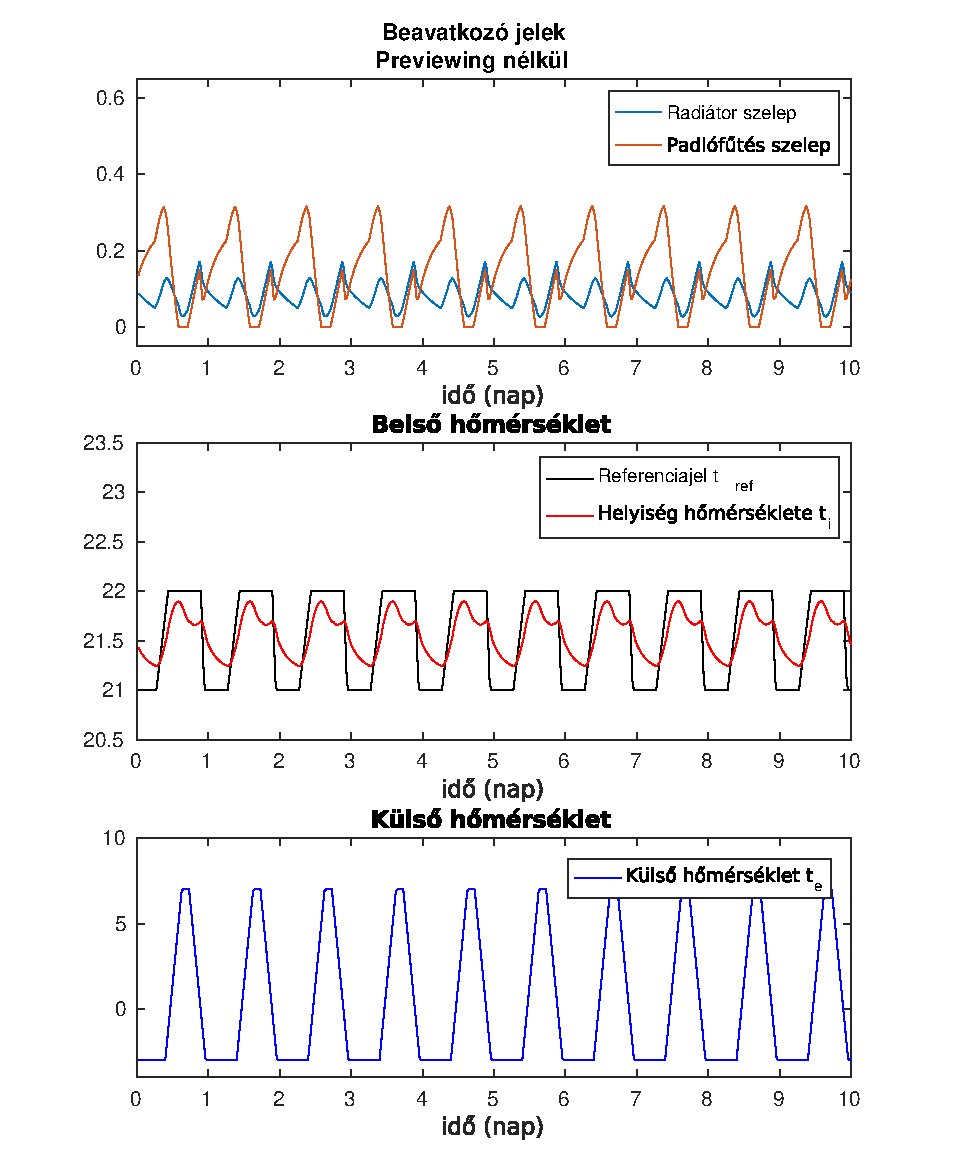
\includegraphics[trim=0 0 0 27, clip,width=\textwidth]{figures/onlab/compare/A_C_P0D0}
		\caption{Preview nélkül}
		\label{fig:mpc-pr0d0}
	\end{subfigure}
	~
	\begin{subfigure}[t]{0.32\textwidth}
		\centering
		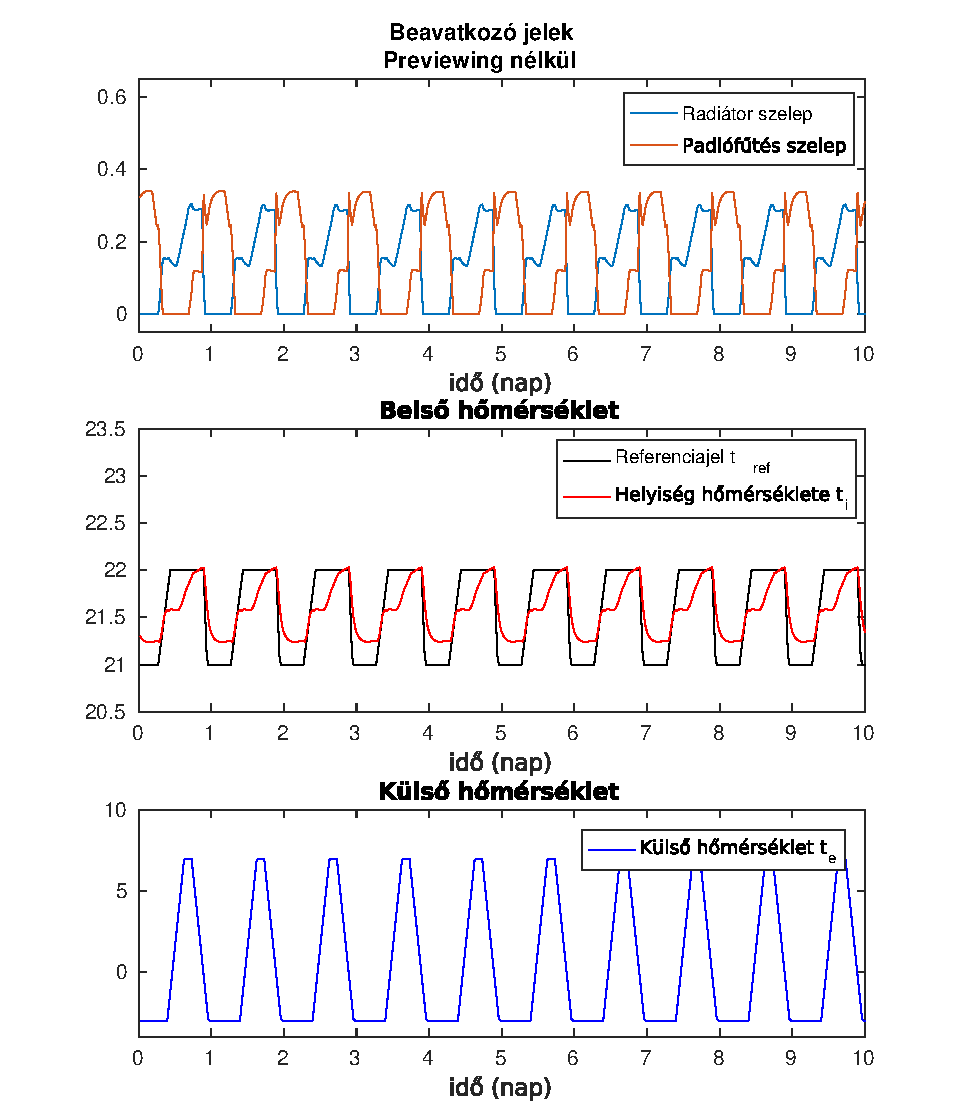
\includegraphics[trim=0 0 0 27, clip,width=\textwidth]{figures/onlab/compare/A_C_P0D10}
		\caption{Disturbance preview 10 step}
		\label{fig:mpc-pr0d10}
	\end{subfigure}
	~
	\begin{subfigure}[t]{0.32\textwidth}
		\centering
		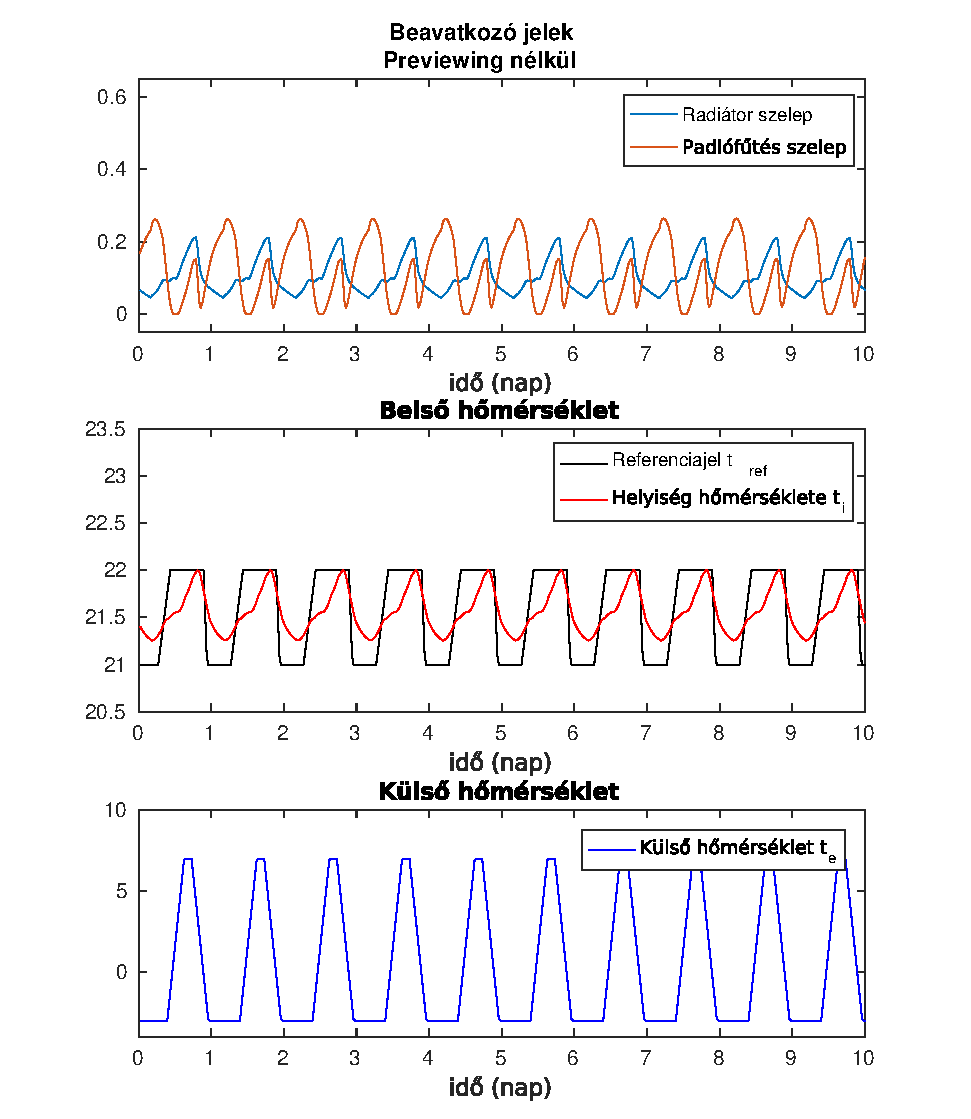
\includegraphics[trim=0 0 0 27, clip,width=\textwidth]{figures/onlab/compare/A_C_P5D10}
		\caption{Reference preview 5 step, disturbance preview 10 step}
		\label{fig:mpc-pr5d10}
	\end{subfigure}
	\caption{MPC viselkedése -- previewing hatása}
	\label{fig:mpc-previeWeight}
\end{figure}


Meg kell jegyezni, hogy a previewing néhány esetben egy siettetést hozott a rendszerbe, azaz még \SI{21}{\celsius}-os alapjel volt előírva, amikor már jóval megemelte a hőmérsékletet. Ha ezeket a követési tulajdonságokat módosítani szeretnénk, érdemes a szabályozó súlyfüggvényében további módosítást végezni.


\begin{figure}[H]
	\begin{subfigure}[t]{0.47\textwidth}
		\centering
		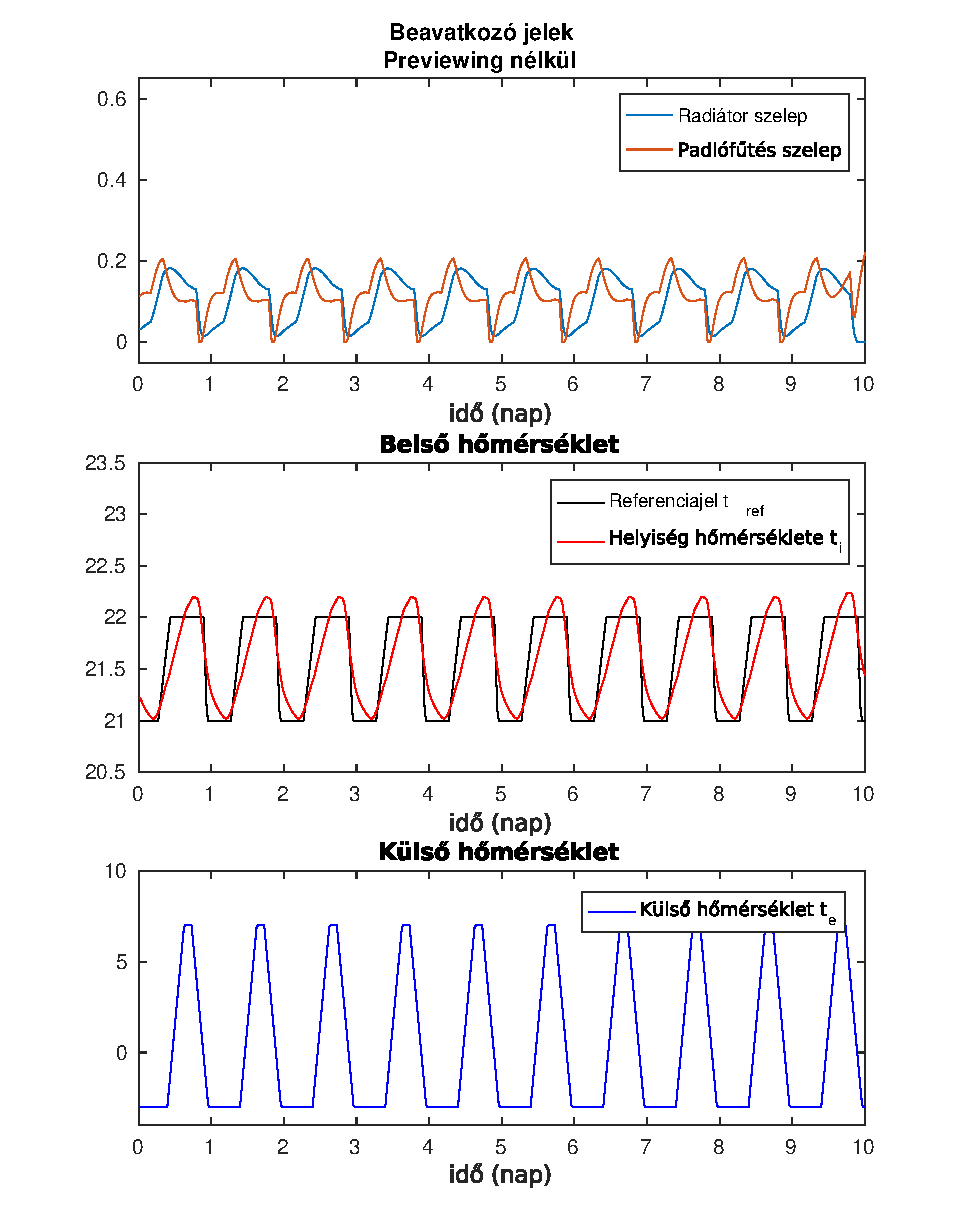
\includegraphics[trim=0 0 0 0, clip,width=\textwidth]{figures/onlab/compare/A_C_P5D48}
		\caption{Preview r5d48}
		\label{fig:mpc-pr5d48}
	\end{subfigure}
	~
	\begin{subfigure}[t]{0.51\textwidth}
		\centering
		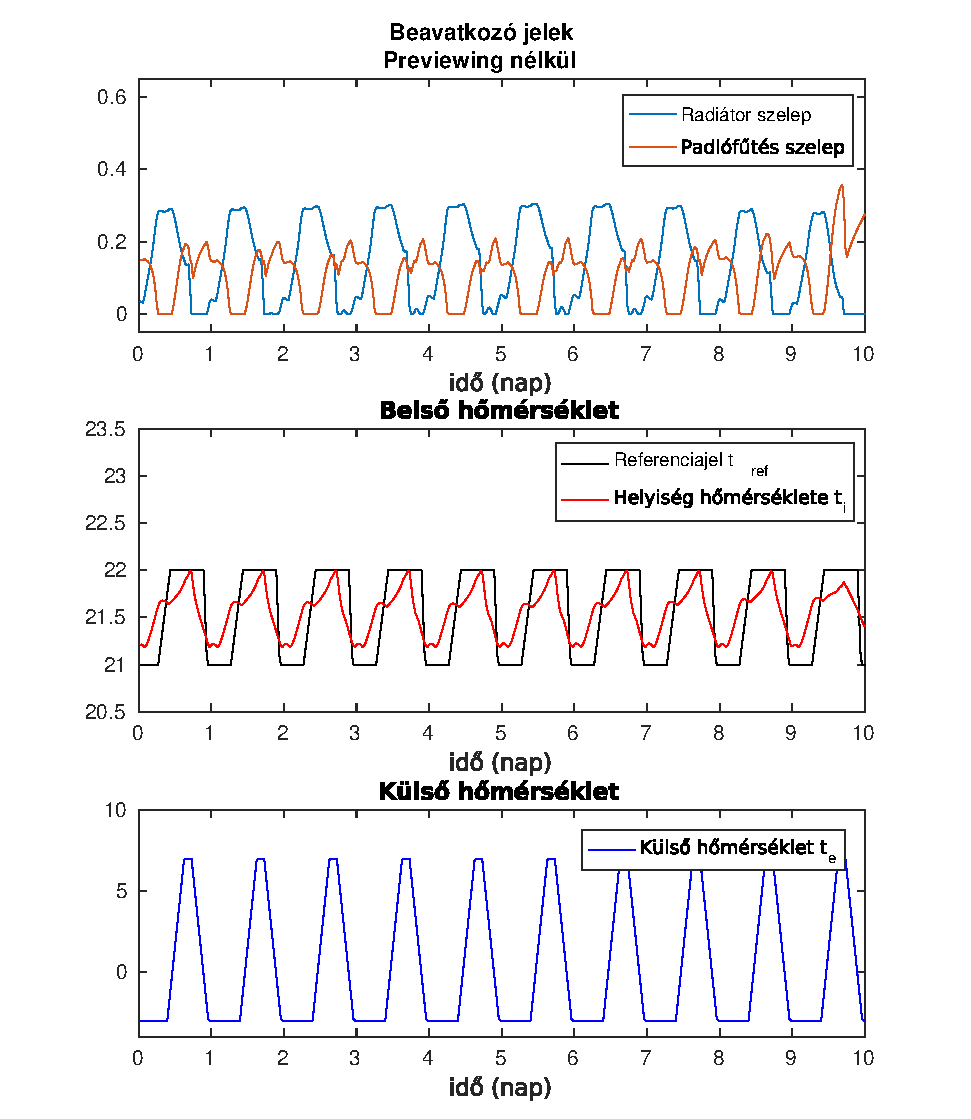
\includegraphics[trim=0 0 0 0, clip,width=\textwidth]{figures/onlab/compare/A_C_P10D48}
		\caption{r10d48}
		\label{fig:mpc-pr10d48}
	\end{subfigure}
\end{figure}


\section{Költségek figyelembe vétele}


A fűtés energiaköltségét legkönnyebben az összes felhasznált energia mennyiségéből kaphatjuk meg. Ezen kívül célszerű még megvizsgálni a maximális teljesítményigényt is (peak demand), illetve az energiaátalakítás teljesítményszintektől függő hatásfokát.

A szimulációban helyiség Simscape modelljéből kivezettem a ténylegesen leadott hőmennyiséget, amiből a radiátoros- és padlófűtés közötti arányra voltam kíváncsi. Abból adódóan, hogy továbi zavarást nem iktattam a rendszerbe, minden szabályozó beállítás mellett az összes energiafelhasználás azonos volt. Valós környezetben történő méréseknél lehetne vizsgálni azt, hogy mely konfiguráció a legelőnyösebb, ezért én csak a módszert mutatom be, ami alapján lehetséges megtalálni az ideális értéket.


\section{Komfort figyelembe vétele}

A szabályozás ezen minőségi jellemzője a hibajellel arányos. Ennek átlaga egy referenciától mért átlagos eltérést ad (ez az állandósult állapotbeli hiba). Ha a hiba abszolút integrálját vesszük, akkor kiválaszthatjuk a zavarokra minimális hibával működő szabályozást. Ezt a mennyiséget Kh, azaz kelvinóra mértékegységben értjük. 

Az alábbi ábrákon látható a költségek és komfort metrikája egyes szabályozókra, a previewing függvényében. (A rövidebb jelölésrendszer érdekében R0 jelöli, ha a referenciajelből csak az aktuális értéket ismerjük, D10 pedig azt, ha a zavarjel (disturbance) értékét 10 lépésre előre ismerjük.)

\begin{figure}[H]
	%	% trim={<left> <lower> <right> <upper>}
	\begin{subfigure}[t]{0.48\textwidth}
		\centering
		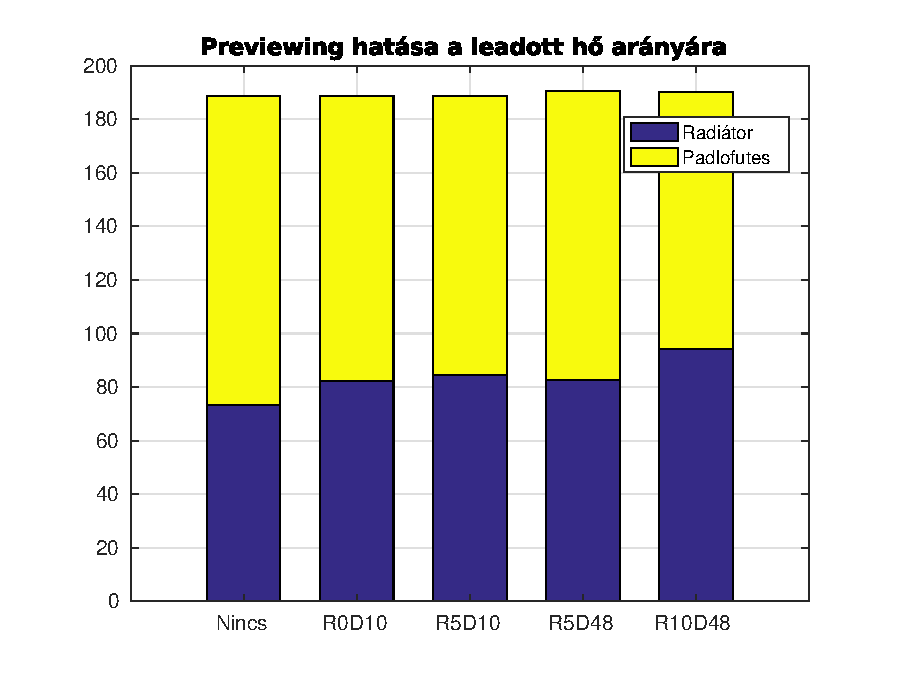
\includegraphics[trim=0 0 0 0, clip,width=1.1\textwidth]{figures/onlab/compare/A_compareEnergy}
		\caption{Leadott homennyiseg megoszlasa}
		\label{fig:constrefHeat}
	\end{subfigure}
	~
	\begin{subfigure}[t]{0.48\textwidth}
		\centering
		\includegraphics[trim=0 0 0 0, clip,width=1.1\textwidth]{figures/onlab/compare/A_compareComfort}
		\caption{C2 szabályozó}
		\label{fig:mpc-PeakDemand}
	\end{subfigure}
\end{figure}

\subsection{Hőérzetbeli különbségek}

A szabályozás performanciáját tovább árnyalja, hogy azonos levegőhőmérséklet esetén is lehet különböző a hőérzetünk. Elég arra gondolni, hogy az időjárás-előrejelzések is megadnak hőérzetet is, amely napsütés esetén a ténylegesnél magasabb, szél esetén alacsonyabb lehet.

A épületekben a sugárzó fűtések magasabb hőérzetet biztosítanak, ezért a referenciajelet alacsonyabbra is lehet állítani.

\section{Súlyozás további hangolása}


